\item[(a)]
\section*{Exercise 3 Task (a): Frequency Analysis of \(x(t)\)}

\subsection*{Objective}
This task involves identifying all positive frequencies up to 20 kHz in the analog signal \(x(t)\), derived from the discrete-time signal \(x[n]\) through a DAC operating at 8 kHz.

\subsection*{Methodology}
The discrete-time signal \(x[n] = \sqrt{2} \cdot \sin\left(2\pi \frac{1}{8} n\right)\) has a fundamental frequency \(f_0 = 1 \text{kHz}\) because it completes \(\frac{1}{8}\) of a cycle per sample, and the DAC operates at 8 kHz. The analysis focuses on the effects of sampling, which replicates the spectrum around multiples of the sampling frequency, leading to potential frequencies at:
\(f_0\),
\(f_s \pm f_0\),
\(2f_s \pm f_0\)
etc., where \(f_s\) is the sampling frequency (8 kHz).

\subsection*{Results}
The positive frequencies identified in \(x(t)\) and shown in Figure~\ref{fig:exercise3a_frequencies} are:
\begin{itemize}
\item 1 kHz (base frequency)
\item 7 kHz (\(8 \text{ kHz} - 1 \text{ kHz}\))
\item 9 kHz (\(8 \text{ kHz} + 1 \text{ kHz}\))
\item 15 kHz (\(16 \text{ kHz} - 1 \text{ kHz}\))
\item 17 kHz (\(16 \text{ kHz} + 1 \text{ kHz}\))
\end{itemize}

\begin{figure}[h]
    \centering
    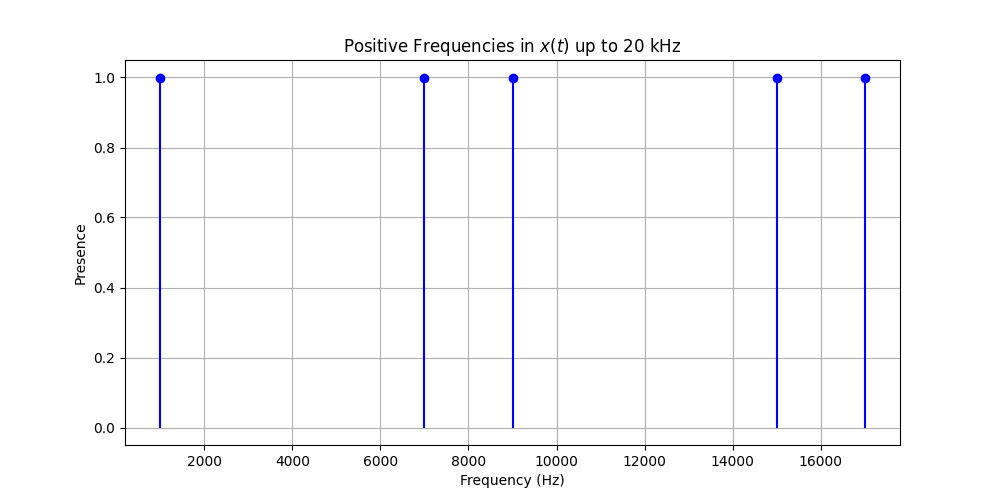
\includegraphics[width=0.8\textwidth]{fig/ex3_task_a_frequencies}
    \caption{Positive frequencies in \(x(t)\) up to 20 kHz}
    \label{fig:exercise3a_frequencies}
\end{figure}

\subsection*{Conclusion}
This detailed frequency analysis underscores the significance of understanding the effects of sampling on the signal's spectrum.
It aids in designing digital systems that effectively manage aliasing and maintain signal fidelity.
